\documentclass{beamer}
\usepackage[T1]{fontenc}
\usepackage[utf8]{inputenc}
\usepackage{hyperref,lmodern}
\usepackage[spanish]{babel}
\usepackage{graphicx}
\mode<presentation>
{
  \usetheme{Warsaw}
  
  \setbeamercovered{transparent}
  
}

\usepackage{times}

\title{Normas de urbanidad en reuniones de campo abierto}

\author[Germán Darío]{Germán Avendaño Ramírez}
% - Use the \inst{?} command only if the authors have different
%   affiliation.

\institute[Universities of Somewhere and Elsewhere] 
{
  \inst{}%
  Colegio Arborizadora Baja I.E.D.
  }
% - Use the \inst command only if there are several affiliations.
% - Keep it simple, no one is interested in your street address.

\date{20 de julio de 2017}

\subject{Talks}

% If you have a file called "university-logo-filename.xxx", where xxx
% is a graphic format that can be processed by latex or pdflatex,
% resp., then you can add a logo as follows:

%\pgfdeclareimage[height=0.5cm]{university-logo}{logo-colegio.png}
%\logo{\pgfuseimage{university-logo}}



% Delete this, if you do not want the table of contents to pop up at
% the beginning of each subsection:

% If you wish to uncover everything in a step-wise fashion, uncomment
% the following command: 

%\beamerdefaultoverlayspecification{<+->}
\hyphenation{Contextua-lización}

\begin{document}

\begin{frame}
  \titlepage
\end{frame}

\begin{frame}{``En los lugares públicos y comunes mucho respeto y prudencia en las acciones''}
  \tableofcontents
  % You might wish to add the option [pausesections]
\end{frame}


% Since this a solution template for a generic talk, very little can
% be said about how it should be structured. However, the talk length
% of between 15min and 45min and the theme suggest that you stick to
% the following rules:  

% - Exactly two or three sections (other than the summary).
% - At *most* three subsections per section.
% - Talk about 30s to 2min per frame. So there should be between about
%   15 and 30 frames, all told.
 \section{Urbanidad}
 \begin{frame}{¿Qué es la urbanidad?}
 La urbanidad es cortesanía, comedimiento, atención y buen modo. Todo esto contribuye a tener una mejor convivencia con los demás. Cualquier sociedad cuenta con unas normas de comportamiento no escritas en la mayor parte de los casos pero que sin su tutela nos haría ser un grupo de seres incivilizados.
 \end{frame}
 \begin{frame}{}
Decir ``perdón'', ``gracias'' y ``por favor'' son fundamentales en el trato con la sociedad.
\end{frame}
\section{Normas} 
\begin{frame}{Primera norma}
\begin{figure}

\includegraphics[scale=.5]{Images/NORMA1.png} 
\end{figure}
La primera norma básica en espacios abiertos es el silencio.
\end{frame}
\begin{frame}{Segunda norma}
\begin{figure}
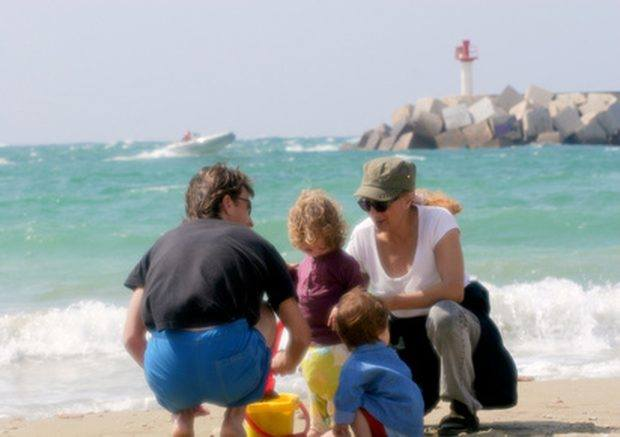
\includegraphics[scale=.35]{Images/NORMA2.png} 
\end{figure}
Si se tienen niños estar pendientes que no molesten a otras personas.
\end{frame}
\begin{frame}{Tercera norma}
\begin{figure}
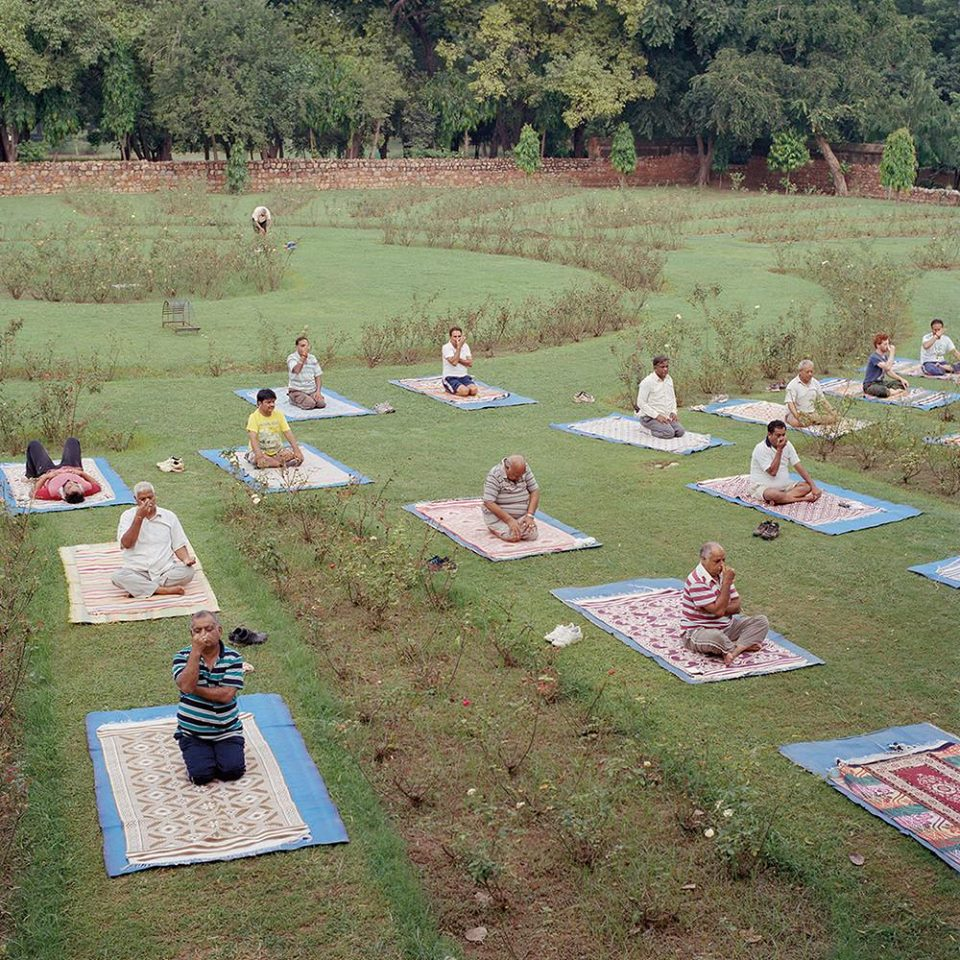
\includegraphics[scale=.175]{Images/NORMA3.png} 
\end{figure}
\begin{center}
Cuidado de no invadir el terreno de otras personas.
\end{center}
\end{frame}
\begin{frame}{Cuarta norma}
\begin{figure}
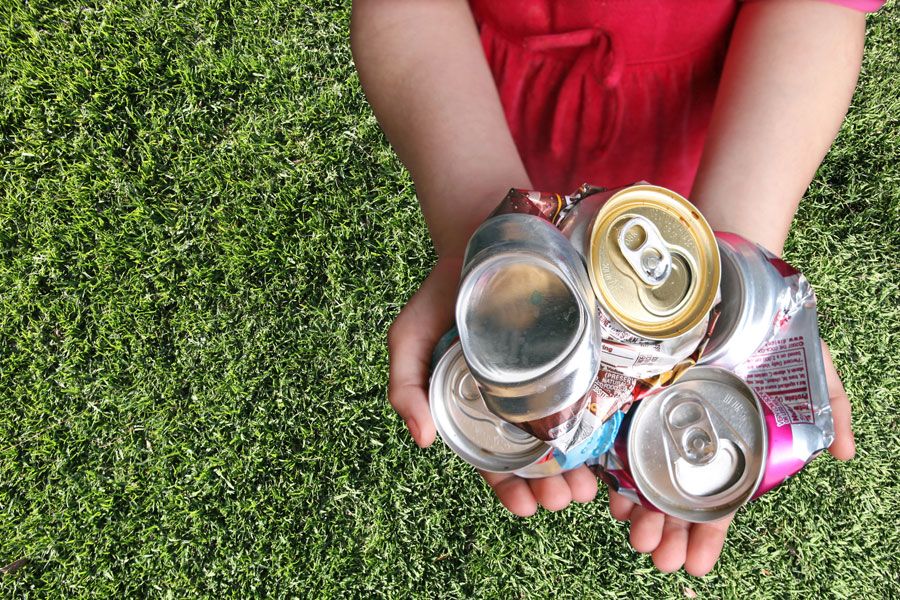
\includegraphics[scale=.25]{Images/NORMA4.jpg}
\end{figure}
\begin{center}
No deben tirarse desperdicios en la calle.
\end{center}
\end{frame}
\begin{frame}{Quinta norma}
\begin{figure}
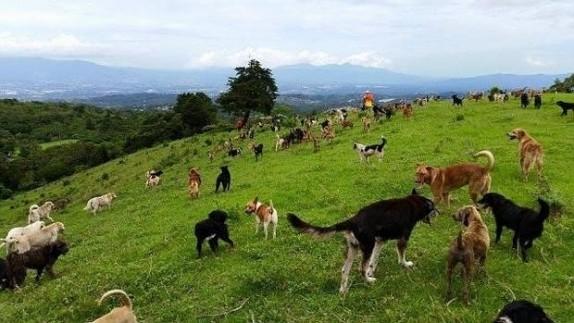
\includegraphics[scale=.5]{Images/NORMA5.jpg} 
\end{figure}
Los animales de compañía deben tener una vigilancia constante y cumplir las reglamentaciones establecidas para ellos.
\end{frame}
\begin{frame}{Sexta norma}
\begin{figure}
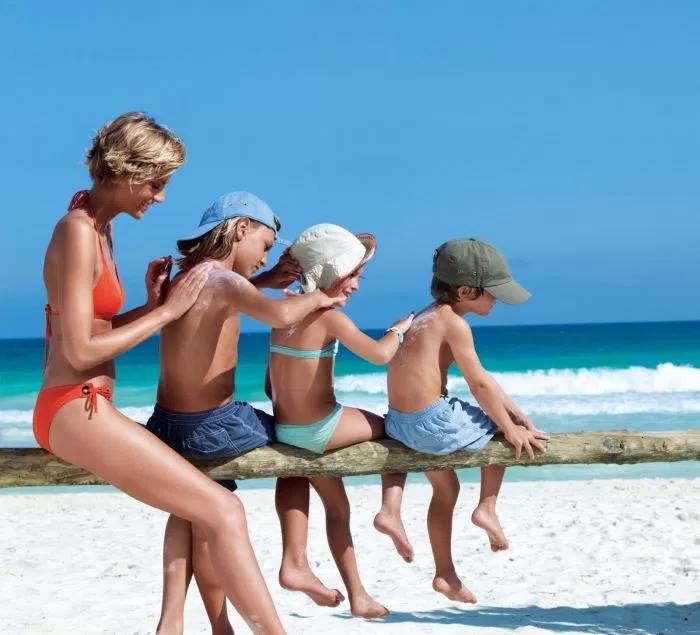
\includegraphics[scale=.25]{Images/NORMA6.png} 
\end{figure}
No se debe utilizar el río o playa como si fuera bañera de casa.
\end{frame}
\begin{frame}{Séptima norma}
\begin{figure}
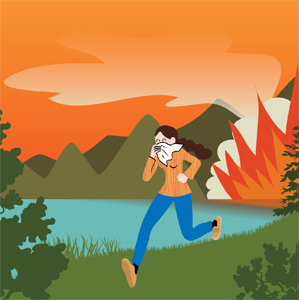
\includegraphics[scale=.55]{Images/NORMA7.jpg} 
\end{figure}
El fuego está totalmente prohibido en la playa y en el campo.
\end{frame}
 \begin{frame}{Octava norma}
 \begin{figure}
 
\includegraphics[scale=.25]{Images/NORMA8.png} 
 \end{figure}
 \begin{center}
 Como se encuentra se deja.
 \end{center}
 \end{frame}
 \begin{frame}{Novena norma}
 \begin{figure}
 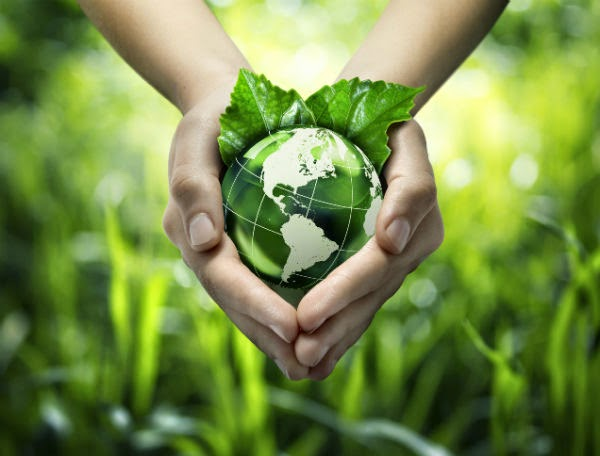
\includegraphics[scale=.35]{Images/NORMA9.jpg} 
 \end{figure}
 El respeto a las demás personas y a la naturaleza en general. 
 \end{frame}
 \begin{frame}
\begin{center}
 Gracias por su atención.
\end{center}
 \end{frame}
\end{document}
